% !TeX spellcheck = cs_CZ
{\tikzset{external/prefix={tikz/FYZI/}}
 \tikzset{external/figure name/.add={ch35_}{}}
%---------------------------------------------------------------------------------------------------
% file fey1ch35.tex
%---------------------------------------------------------------------------------------------------
%=========================== Kapitola: Barevné vidění =============================================
\chapter{Barevné vidění}\label{fyz:IchapXXXV}
\minitoc
  \section{Lidské oko}\label{fyz:IchapXXXVsecI}
    Existence barev závisí zčásti na fyzikálním světě. O barvách mýdlových bublin a podobných 
    jevech mluvíme jako o výsledku interference. Existence barev, samozřejmé, závisí na oku a na 
    tom, co se děje za okem, v mozku. Fyzika charakterizuje světlo vstupující do oka, ale dále jsou 
    naše vjemy výsledkem fotochemicko-neurologických procesů a psychologické odezvy.
    
    Existuje mnoho zajímavých jevů spojených s viděním, jež zahrnují směs fyzikálních jevů a 
    fyziologických procesů a jejich úplné pochopení musí sahat za hranice fyziky v obvyklém smyslu. 
    Nechceme se omlouvat za takové odbočení do jiných oblastí poznání, neboť rozdělení do různých 
    oblastí je pouhá lidská konvence a nepřirozená věc. Přírodu nezajímá naše dělení a mnoho 
    zajímavých jevů překlenuje mezery mezi různými oblastmi.
   
    Třetí kapitolu jsme věnovali obecným vztahům mezi fyzikou a jinými vědními obory a nyní se 
    podrobněji podíváme na jednu oblast, v níž mají fyzika a jiné vědy k sobě velice, velice 
    blízko. Tato oblast se týká \emph{vidění}. Přesněji, budeme mluvit o \emph{barevném vidění}. V 
    této kapitole se soustředíme hlavně na pozorovatelné jevy lidského vidění a v následující 
    kapitole na fyziologické aspekty vidění jak u člověka, tak u jiných živočichů.
    
    Vše začíná okem. Abychom pochopili vidění, potřebujeme jisté znalosti o oku. V další kapitole 
    se budeme zabývat tím, jak pracují jednotlivé části oka a jak jsou navzájem propojeny s 
    nervovým systémem. Teď si jen stručně popíšeme funkci oka (obr. \ref{fyz:fig130a}).

    \begin{figure}[ht!]  %\ref{fyz:fig130}
      \centering
      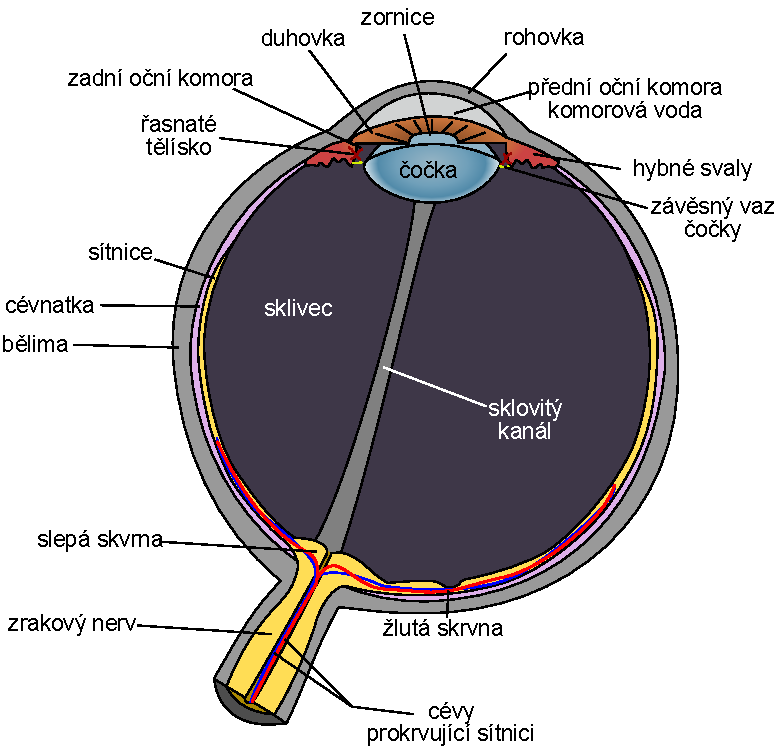
\includegraphics[width=0.8\linewidth]{fyz_fig130a.pdf}
      \caption{Oko: Rohovka (cornea), duhovka (iris), čočka (lens), řasnatá vlákna, bělmo 
              (sclera), spojivka, kruhový sval (ciliari muscle), sklivec (vitreous), sítnice 
              (retina), cévnatka (choroid), oční svaly, žlůtá skvrna (macula lutea), zrakový 
              nerv (optic nerve) 
              (\cite[s.~468]{Feynman01})}
      \label{fyz:fig130a}
    \end{figure} 

    Světlo vstupuje do oka \textbf{rohovkou}. Již jsme mluvili o tom, jak se přitom láme a jak se 
    vytváří obraz na sítnici umístěné v zadní částí oka, takže na ni dopadá světlo z různých částí 
    vnějšího zorného pole. \textbf{Sítnice} není úplně stejnorodá. Existuje na ní místo, jež se 
    nazývá \textbf{žlutá skvrna}. Leží ve středu zorného pole, kde vidíme nejostřeji a používáme 
    ji, když si chceme něco důkladně prohlédnout. Z naší zrakové zkušeností dobře víme, že pro 
    rozeznání detailů jsou okrajové části oka podstatně méně účinné než jeho střed. Na sítnici je 
    také místo, odkud vycházejí nervy přenášející zrakové informace; je to \textbf{slepá skvrna}. 
    Na ní se nenacházejí žádné citlivé částí sítnice. Můžeme se o ní přesvědčit například tak, že 
    když zavřeme levé oko díváme se přímo na nějaký předmět a pak začneme posouvat prst nebo nějaký 
    jiný malý předmět ven ze zorného pole, najednou ho v jisté poloze neuvidíme. 
    
    \begin{figure}[ht!]  %\ref{fyz:fig131}
      \centering
      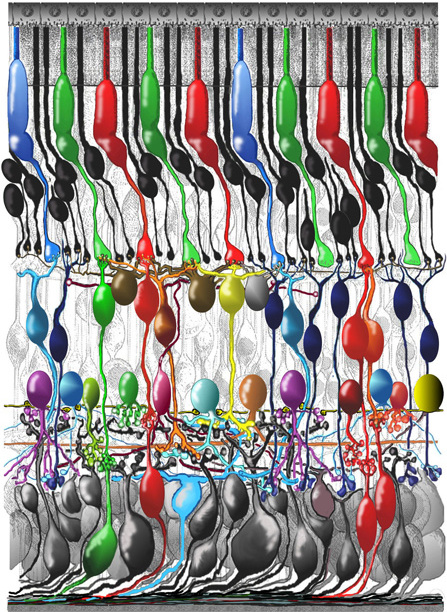
\includegraphics[width=0.9\linewidth]{fyz_fig131_rev1.jpg}
      \caption{Pohled na strukturu lidské \WebvisionRetina 
               (\cite[s.~468]{Feynman01}, \cite{Webvision})}
      \label{fyz:fig131}
    \end{figure}
    Na obrázku \ref{fyz:fig131} je ve zvětšeném měřítku schematicky znázorněn průřez sítnicí. V 
    různých částech má sítnice různou strukturu. Na okraji sítnice je nejvíc buněk, jež se nazývají 
    \textbf{tyčinky}. V blízkosti žluté skvrny najdeme u tyčinek i \textbf{čípky}. Jejich strukturu 
    si popíšeme později. Čím blíže k žluté skvrně, tím je větší počet čípků a v samotné žluté 
    skvrně jsou už jen tyto buňky. Jsou tam tak nahuštěny, že jsou mnohem jemnější nebo tenčí než 
    kdekoliv jinde na sítnici. Znamená to, že ve středu zorného pole vidíme pomocí čípků, ale 
    směrem k okraji jsou rozloženy tyčinky. Zajímavé je, že každá buňka sítnice citlivá ke světlu 
    není spojena vláknem přímo s optickým nervem, aleje spojena s mnoha jinými buňkami, jež jsou 
    tak navzájem propojeny. Jsou to v podstatě \(4\) druhy buněk; některé přenášejí informace na 
    optický nerv, jiné jsou pospojovány hlavně „horizontálně“. Nyní se však nebudeme pouštět do 
    takových detailů. Hlavní, co zdůrazňujeme, je, že světelný signál se již zde zpracovává. 
    Informace z různých buněk se nedostávají přímo do mozku, bod po bodu, ale v sítnici dochází ke 
    zpracování určité části informace pomocí kombinace informací z různých zrakových receptorů. Je 
    důležité, abychom si uvědomili, že určité jevy spojené s mozkovou činností probíhají již v 
    samotném oku.
    
  \section{Barva závisí na intenzitě}\label{fyz:IchapXXXVsecII}
    Jednou z nejpřekvapivějších vlastností vidění je adaptace oka na tmu. Když vyjdeme z 
    rozsvíceného pokoje do tmy, vidíme chvíli velmi špatně, ale postupně lépe a lépe, až nakonec 
    vidíme předměty, které jsme předtím vůbec neviděli. Při velmi malé intenzitě osvětlení, věci, 
    které vidíme, nemají barvu. Je známo, že vidění přizpůsobené tmě je téměř zcela zprostředkováno 
    tyčinkami, zatímco vidění v jasném světle je zprostředkováno čípky. Tak tedy můžeme pochopit 
    mnohé jevy jako důsledek přechodu od společné funkce tyčinek a čípků k samotné funkci tyčinek.
    
    \begin{figure}[ht!]  %\ref{fyz:fig132}
      \centering
      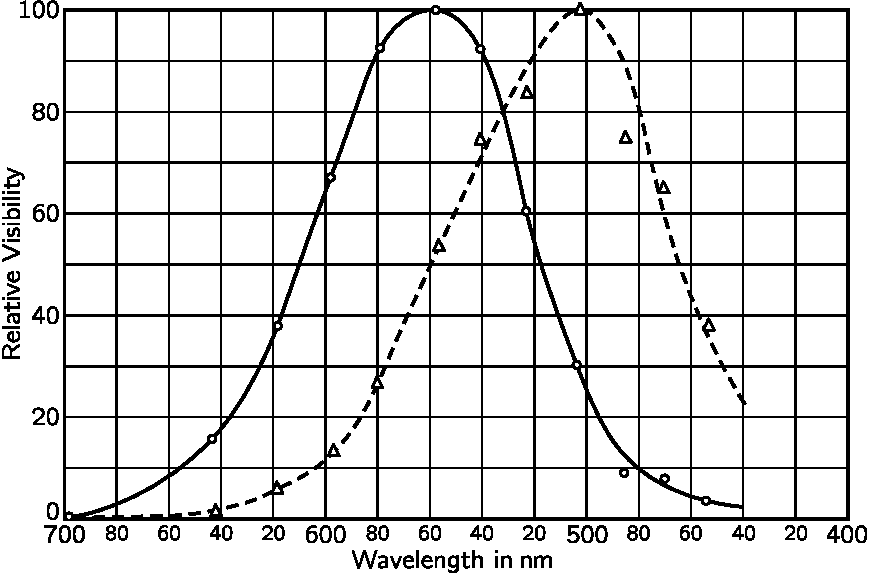
\includegraphics[width=0.95\linewidth]{fyz_fig132.pdf}
      \caption{Spektrální citlivost oka. Přerušovaná čára odpovídá tyčinkám, plná čára odpovídá 
               čípkům
               (\cite[s.~470]{Feynman01})}
      \label{fyz:fig132}
    \end{figure}
    V mnoha případech, kdyby intenzita světla byla větší, bychom viděli barvy a zjistili bychom, že 
    věci, které vidíme, jsou krásné. Například při pohledu teleskopem vidíme obrazy nejasných 
    mlhovin jako černobílé. W. C. Miller v observatořích na Mt Wilsonu a Mt Palomaru měl dostatek 
    trpělivosti, aby získal barevné snímky takových objektů. Nikdo nikdy okem tyto barvy neviděl, 
    ale nejsou to umělé barvy, je to prostě dáno tím, že intenzita světla není dostatečná k tomu, 
    abychom ho viděli čípky v našem oku. Mezi nejokázalejší objekty tohoto druhu patří Prstencová 
    mlhovina a Krabí mlhovina. První má vnitřní část krásně modrou s jasně červeným vnějším kolem a 
    druhá má modrý opar prostoupený jasně červeno - oranžovými vlákny.
    
    V jasném světle mají tyčinky velmi malou citlivost, ale ve tmě se časem jejich schopnost vidět 
    světlo zvětšuje. Změny intenzity světla, na které je možno se adaptovat, jsou ve větším poměru 
    než milión ku jedné. Tato adaptace se v přírodě neděje jen pomocí buněk jednoho druhu, ale 
    funkce vidění se posouvá od buněk citlivých na jasné světlo, vidících barvy, tj. čípků, k 
    tyčinkám - buňkám citlivým k malým intenzitám a přizpůsobivým šeru. Mezi zajímavé důsledky 
    tohoto posunu patří, za prvé, že se vytratí barva a za druhé, že různě zbarvené předměty mají 
    různý relativní jas. Ukazuje se, že tyčinky vidí lépe než čípky směrem k modré barvě a čípky 
    vidí například červené světlo, zatímco pro tyčinky to je absolutně nemožné. Proto je červené 
    světlo pro tyčinky černé. Dva barevné papíry, řekněme modrý a červený, přičemž červená barva 
    může být na dobrém světle jasnější než modrá, se budou v přítmí, co se týká jasnosti, jevit 
    zcela naopak. Je to velmi překvapující jev. Když si v tmavé místnosti prohlédneme barevný 
    časopis nebo jiný barevný předmět, můžeme posoudit, které plochy jsou světlejší, a které jsou 
    tmavší, a když ho pak vyneseme na světlo, uvidíme, jak zajímavě se mění jasnost toho, co se 
    zdálo být nejjasnější, a co se nezdálo být tak jasné. Tento jev se nazývá \emph{Purkyňův efekt}
    
    Na obrázku \ref{fyz:fig132} máme křivky citlivosti oka v přítmí; přerušovaná čára odpovídá 
    situaci, kdy používáme tyčinky, zatímco plná čára znázorňuje citlivost oka za světla. Vidíme, 
    že tyčinky jsou nejcitlivější pro zelenou oblast a čípky pro žlutou oblast. Červeně zabarvený 
    papír (\SI{650}{\nm}) vidíme, když je dobře osvětlený, ale ve tmě ho skoro nevidíme.
    
    Dalším projevem toho, že v přítmí přebírají funkci vidění tyčinky, a že ty nejsou ve žluté 
    skvrně, je fakt, že díváme-li se v přítmí přímo na nějaký předmět, nevidíme ho tak ostře, jako 
    když se na něj podíváme trochu z boku. Nejasnou hvězdu nebo mlhovinu můžeme někdy lépe vidět, 
    když se na ni podíváme mírně ze strany, než když se na ní díváme přímo, protože ve středu žluté 
    skvrny nemáme citlivé tyčinky.
    
    Jiným zajímavým důsledkem toho, že směrem k okraji zorného pole počet čípků klesá, je 
    skutečnost, že dokonce jasně zbarvené předměty přitom ztrácejí svou barvu. Přesvědčit se o tom 
    je možné tak, že se díváme v určitém neměnném směru a necháme, aby se někdo, kdo drží v ruce 
    nějaký barevný předmět, přibližoval do směru našeho pohledu ze strany. Dříve než se dostane 
    přímo před nás, snažme se rozhodnout, jakou barvu má daný předmět. Zjistíme, že předmět vidíme 
    mnohem dřív, než jsme schopni určit jeho barvu. Doporučuje se vstupovat do zorného pole z 
    opačné strany než je slepá skvrna, neboť jinak vzniká zmatek; nejdříve už téměř vidíme barvu, 
    pak najednou nevidíme nic a pak opět vidíme barvu.
    
    Další zajímavostí je, že okrajové části sítnice jsou velmi citlivé k pohybu. I když koutkem oka 
    dobře nevidíme, když se na kraji našeho zorného pole pohne nějaký malý brouček, o němž ani 
    nevíme, že tam je, ihned to zaregistrujeme. Všichni jsme stvořeni tak, že ostražitě vnímáme, 
    když se něco pohne na okraji našeho zorného pole.
    
  \section{Měření barevného vjemu}\label{fyz:IchapXXXVsecIII}
    Nyní přejdeme k vidění za jasného světla, k vidění pomocí čípků a k otázce barvy, jež je pro 
    toto vidění nejcharakterističtější. Jak víme, bílé světlo je možné rozložit pomocí hranolu na 
    celé spektrum vlnových délek, které vnímáme jako různé barvy. Barvy, to jsou naše vjemy. 
    Libovolný zdroj světla lze analyzovat pomocí difrakční mřížky nebo pomocí hranolu a lze určit 
    jeho spektrální složení, tj. „množství“ světla každé vlnové délky. Některé světlo může 
    obsahovat mnoho modré barvy, dost červené, málo žluté atd. Fyzikálně lze vše určit velmi 
    přesně, otázkou však je, jakou barvu budeme vnímat. Je samozřejmé, že různé barvy nějak závisí 
    na spektrálním složení světla, problém je v tom, jaké spektrální charakteristiky způsobí různé 
    barevné vjemy. Například, co je třeba udělat, abychom viděli zelenou barvu? Všichni víme, že 
    prostě stačí vzít si zelenou část spektra. Je to však jediný způsob, jak lze získat zelenou 
    nebo jakoukoliv jinou barvu?
    
    Existuje více spektrálních rozložení, jež způsobí stejný vizuální efekt? Určitě ano. Jak brzy 
    uvidíme, počet základních vizuálních efektů je velmi omezen, fakticky jsou jen tři, ale 
    existuje nekonečné množství různých spektrálních křivek, jež můžeme nakreslit pro světlo 
    přicházející z různých zdrojů. Potřebujeme vyřešit tuto otázku: Za jakých podmínek se různé 
    rozložení světla jeví oku jako stejná barva?
    
    Nejúčinnější psychofyzikální technikou k určení barev je ta, když se oko používá jako nulový 
    přístroj. Přitom se nesnažíme definovat, co způsobuje, že barvu vnímáme jako zelenou, nebo za 
    jakých okolností k tomu dochází. To by bylo příliš složité. Místo toho studujeme, za jakých 
    podmínek jsou dva vizuální podněty nerozlišitelné. Pak nemusíme rozhodovat, zda dva lidé vidí 
    stejné vjemy za různých okolností, ale spíš jen to, zda budou dva vjemy stejné pro jednu osobu 
    stejné i pro osobu jinou. Nemusíme rozhodnout, zda to, co někdo cítí, když vidí něco zeleného, 
    je stejné jako to, co cítí jiný při pohledu na stejnou věc. O tom stejně nic nevíme.
    
    Pro ilustraci těchto možností můžeme použít čtyři projektory s filtry, jejich jas lze spojitě 
    měnit v širokém rozmezí. Jeden má červený filtr a na plátně vytvoří červenou skvrnu, druhý má 
    zelený filtr a vytváří zelenou skvrnu, třetí má modrý filtr a čtvrtý vytváří bílý kruh s černou 
    skvrnou uprostřed. Zapneme-li nyní červené světlo a dále zelené, vidíme, že část, kde se barvy 
    překrývají, v nás vyvolá vjem, který nenazýváme červeno - zelenou barvou, ale nové, v tomto 
    případě žluté barvy. Změnou proporcí červené a zelené můžeme projít různými odstíny oranžové 
    atd. Nastavíme-li filtry na určitý odstín žluté, můžeme tentýž odstín získat, dostat ne 
    smísením těchto dvou barev, ale smísením některých jiných barev, například žlutého filtru a 
    bílého světla nebo něčeho podobného, co vytváří stejný vjem. Takže různé barvy lze vytvářet 
    nejen jedním způsobem, ale více způsoby, míšením barev z různých filtrů.
    
    Tento náš objev lze vyjádřit analyticky. Například určitou žlutou barvu lze vyjádřit jako 
    nějaký symbol \(Y\), jenž je součtem určitého množství světla z červeného filtru (\(R\)) a ze 
    zeleného filtru (\(G\)). Když k popisu jasu světla (\(R\)) a (\(G\)) použijeme písmena \(r\) a  
    \(g\), máme pro žluté světlo
    \begin{equation}\label{FYZ:eq234}
      Y = rR + gG.
    \end{equation}
    Jak můžeme získat všechny různé barvy smísením dvou nebo tří světel různých pevně zvolených 
    barev? Podívejme se, co lze v této souvislosti udělat. Všechny barvy určitě nezískáme jen 
    smísením červené a zelené, neboť tato kombinace například nikdy nedá modrou. Když k nim přidáme 
    modrou, střední část, kde se všechny tři barvy prolínají, lze zbarvit tak, že je skoro bílá. 
    Sledováním střední částí při míšení těchto různých barev zjistíme, že změnou jejich proporcí 
    můžeme získat pozoruhodné spektrum barev a není vyloučeno, že smísením těchto tří barev je 
    možné vytvořit všechny barvy. Povíme si, do jaké míry je to pravda; v podstatě je to tak a brzy 
    uvidíme, jak lépe definovat jejich proporce.
    
    Abychom to lépe objasnili, nastavíme projektory tak, aby se všechny skvrny vzájemně překrývaly, 
    a pak se pokusíme smísením dostat barvu, kterou bude mít vnější prstenec při zapnutí čtvrté 
    lampy. To, co jsme považovali za bílou barvu čtvrtého projektoru, se teď jeví nažloutlé. 
    Vhodnými změnami intenzity červené, zelené a modré barvy můžeme po několika pokusech najít 
    barvu, která se velmi blíží k tomuto odstínu „krémové“, jakou má prstenec. Proto není těžké 
    uvěřit, že můžeme vytvořit všechny barvy. Za chvíli se pokusíme udělat žlutou barvu, ale 
    nejdřív si řekneme, že existuje barva, jejíž vytvoření může být velmi obtížné. Lidé, kteří 
    přednášejí o barvách, vytvářejí všechny možné barvy, ale nikdy ne \emph{hnědou} a je dost těžké 
    si vzpomenout, zda jsme vůbec někdy viděli hnědé světlo. Co se toho týká, tato barva se nikdy 
    nepoužívá při vytváření světelných efektů na jevištích, takže se zdá, že vytvořit hnědé světlo 
    může být nemožné. Abychom zjistili, zda lze hnědé světlo vytvořit, poznamenáme, že hnědé světlo 
    je něco, co nejsme zvyklí vidět bez příslušného pozadí. Fakticky ho můžeme sestavit smísením 
    červené a žluté. Na důkaz toho, že se díváme na hnědé světlo, prostě zvýšíme jas pozadí, proti 
    kterému se na světlo díváme a zjistíme, že je to skutečně to, co nazýváme hnědou! Hnědá, to je 
    vždy tmavá barva na světlejším pozadí. Hnědou barvu můžeme snadno měnit. Když dáme například 
    pryč trochu zelené, dostaneme červenohnědou jako je barva čokolády, a když přidáme trochu 
    zelené, dostaneme tu strašnou barvu, jakou mají uniformy americké armády, ale světlo této barvy 
    není tak strašné samo o sobě; když ho vidíme proti světlému pozadí, je žlutavě zelené.
    
    Nyní dejme na čtvrtou lampu žlutý filtr a pokusme se takovou barvu namísit. (Samozřejmě, že 
    intenzita musí být v rozsahu jednotlivých lamp. Nemůžeme namísit příliš jasnou barvu, neboť 
    lampy nemusí mít dostatečný výkon.) Žlutou však namísit můžeme. Použijeme směs zelené a červené 
    a k tomu přidáme špetku modré, aby to bylo perfektní. Snad jsme ochotni věřit, že při dobrých 
    podmínkách můžeme dokonale namísit jakoukoliv danou barvu.
    
    Nyní si proberme zákony míšení barev. V první řadě jsme zjistili, že různá spektrální složení 
    mohou vytvářet stejnou barvu. Dále jsme zjistili, že „libovolnou“ barvu lze vytvořit smísením 
    tří barev - červené, modré a zelené. Nejzajímavější rys míšení barev je tento: Máme-li nějaké 
    barevné světlo, řekněme \(X\), které je pro oko nerozlišitelné od světla \(Y\) (může mít jiné 
    spektrální složení, ale \emph{jeví} se jako nerozlišitelné), nazýváme tato světla „stejnými“ v 
    tom smyslu, že oko je; vnímá jako stejná a píšeme
    \begin{equation}\label{FYZ:eq229}
      X = Y.
    \end{equation}
    Zde máme jeden z velkých zákonů barev: Jsou-li dvě spektrální složení nerozlišitelná a 
    přidáme-li ke každému z nich, řekněme, světlo \(Z\) (zápis \(X+ Z\) znamená, že obě světla 
    svítí na stejné místo) a pak vezmeme \(Y\) a přidáme k němu stejné množství stejného světla 
    \(Z\), nové směsi jsou též navzájem nerozlišitelné
    \begin{equation}\label{FYZ:eq230}
      X + Z = Y + Z.
    \end{equation}
    Před chvílí jsme namísili žlutou barvu, aby odpovídala předloze. Osvítíme-li ji spolu s 
    předlohou růžovým světlem, nové barvy si budou opět odpovídat. Takže přidání jakéhokoliv světla 
    k barvám, které již jsou stejné, zanechá opět stejné barvy. Mohli bychom to shrnout tak, že 
    máme-li jednou světla, která se barevně rovnají, když je vidíme vedle sebe a za stejných 
    podmínek, jejich rovnost se zachová a jedno světlo můžeme zaměnit druhým při libovolném míšení 
    barev. Fakticky se ukazuje, a je to velmi důležité a zajímavé, že tato rovnost barev světla 
    nezávisí na charakteristikách oka v době pozorování. Víme, že když se dlouho díváme na jasnou 
    červenou plochu nebo do jasného červeného světla, a pak se podíváme na bílý papír, zdá se být 
    zelenkavý a i ostatní barvy vidíme pozměněny. Když však máme nyní dvě stejná, řekněme, žlutá 
    světla, jež skutečně vnímáme jako stejná, pak se nadlouho zahledíme na jasnou červenou plochu, 
    a opět se podíváme zpět na naše žluté barvy, už nebudou vypadat jako žluté. Nevím, jak budou 
    vypadat, ale přesto se budou jevit stále stejné. Proto, když se oko přizpůsobuje různé 
    intenzitě světla, rovnost barev stále platí se zřejmou výjimkou, když se dostaneme do oblasti, 
    kde je intenzita světla tak malá, že vidění se přesouvá z čípků na tyčinky. Pak už rovnost 
    barev neplatí, neboť používáme jiný systém.
    
    Druhý princip týkající se míšení barev je tento: Jakoukoliv barvu lze vytvořit ze tří různých 
    barev, v našem případě z červené, zelené a modré. Jejich míšením ve vhodném poměru můžeme 
    vytvořit barvu, jakou chceme, jak jsme si ukázali na našich dvou příkladech. Tyto zákony jsou 
    velmi zajímavé i matematicky. Předpokládejme, že vezmeme naše tři barvy, červenou, zelenou a 
    modrou, označíme je jako \(A\), \(B\), \(C\) a budeme je nazývat našimi \emph{primárními 
    barvami}. Každou barvu pak lze vytvořit smísením těchto tří barev v určitých množstvích; 
    například množství \(a\) barvy \(A\) plus množství \(b\) barvy \(B\) a množství \(c\) barvy 
    \(C\) dává barvu \(X\)
    \begin{align}
      X &= aA + bB + cC.     \label{FYZ:eq231}     \\
      \shortintertext{Předpokládejme, že jinou barvu lze vytvořit ze stejných barev.}
      Y &= a'A + b'B + c'C.  \label{FYZ:eq232}
    \end{align}
    Pak se ukazuje, že smísením těchto dvou světel se získá světlo, jež lze vytvořit tak, že 
    sčítáme složky \(X\) a \(Y\) (je to jeden z důsledků zákonů, o nichž jsme právě mluvili):
    \begin{equation}\label{FYZ:eq233}
      Z = X + Y = (a+a')A + (b+b')B + (c+c')C.
    \end{equation}
    Vypadá to jako matematika sčítání vektorů, kde \((a, b, c)\) jsou souřadnice jednoho vektoru a 
    \((a‘, b‘ c')\) jsou souřadnice druhého vektoru, přičemž nové světlo \(Z\) je „součtem“ těchto 
    vektorů. To je předmět, který vždy přitahoval fyziky i matematiky. Například Schr{\"o}dinger 
    napsal o barevném vidění nádherný článek, v němž rozvinul tuto teorii vektorů k analýze míšení 
    barev.
    
    Vzniká otázka, které primární barvy jsou správné. Něco takového jako správné primární barvy k 
    míšení světla neexistuje. Z praktického hlediska mohou existovat tři barevné pigmenty, z nichž 
    lze namíchat víc barevných odstínů a jež jsou užitečnější než jiné tři, ale to nás nyní 
    nezajímá. Libovolná tři různě barevná světla\footnote{ Samozřejmě s výjimkou případu, kdy barva 
    jednoho z nich vznikne smísením barev druhých dvou. } lze vždy smísit ve správném poměru a 
    vznikne jakákoliv jiná barva. Můžeme předvést tento fantastický fakt? Místo červené, zelené a 
    modré použijeme v našich projektech červenou, modrou a žlutou. Můžeme použít červenou, modrou a 
    žlutou k vytvoření dejme tomu zelené?
    
    Míšením těchto tří barev v různých poměrech dostáváme různé barvy v rozsahu téměř celého 
    spektra, ale přes mnohé pokusy zjistíme, že nic z toho se nepodobá zelené. Otázka zní: „Můžeme 
    vytvořit zelenou?“ Ano, ale jak? Když do zelené přimícháme trochu červené, vznikne barva, 
    kterou můžeme vytvořit pomocí určitého poměru žluté a modré! Takže nakonec jsme dosáhli 
    rovnosti barev, jenomže jsme museli udělat malý podvod tím, že jsme přidali červenou na druhou 
    stranu. Protože však máme určitou matematickou představu, chápeme, že jsme vlastně dokázali 
    nikoliv to, že \(X\) lze vždy vytvořit, dejme tomu, z červené, modré a žluté, ale přidáním 
    červené na druhou stranu jsme zjistili, že červená plus \(X\) se dá vytvořit z modré a žluté. 
    Převedení červené na druhou stranu rovnice, můžeme interpretovat jako záporný příspěvek, takže 
    dovolíme-li, aby koeficienty v rovnici, jako je (\ref{FYZ:eq231}), byly jak kladné tak i 
    záporné, a interpretujeme-li záporný příspěvek tak, že znamená přidání dané barvy na druhou 
    stranu, můžeme tvrdit, že jakoukoliv barvu lze vytvořit libovolnými třemi barvami a něco 
    takového jako fundamentální primární barvy neexistuje.
    
    Můžeme se zeptat, zda existují takové tři barvy, z nichž lze získat všechny ostatní jen pomocí 
    kladných příspěvků. Odpověď je, že neexistují. Každá sada tří primárních barev vyžaduje pro 
    některé barvy záporné příspěvky, a proto neexistuje jediný způsob, jak definovat primární barvy.
    V základních učebnicích se říká, že jsou to červená, zelená a modrá, ale to je dáno jen tím, že 
    z těchto barev lze získat větší spektrum barev jen pomocí kladných příspěvků než pro některé 
    jiné kombinace.
    
  \section{Diagram barevnosti}\label{fyz:IchapXXXVsecIV}
    Nyní se podívejme na kombinace barev na úrovni matematiky v geometrickém vyjádření. Je-li možné 
    každou barvu reprezentovat rovnicí (\ref{FYZ:eq231}), můžeme ji znázornit jako vektor v 
    prostoru, kde na osy barevných souřadnic nanášíme hodnoty \(a\), \(b\) a \(c\) a určité barvě 
    odpovídá určitý bod. Odpovídají-li jiné barvě jiné hodnoty \((a‘, b‘, d‘,)\), odpovídá jí jiný 
    bod. Smísením těchto dvou barev vznikne barva, kterou získáme sčítáním těchto dvou vektorů. 
    Tento diagram lze do roviny zjednodušit na následujícím základě: zdvojnásobíme-li pro nějakou 
    barvu \(a\), \(b\) a \(c\), tj. když je všechny zvětšíme ve stejném poměru, dostaneme stejnou 
    barvu jen jasnější.
    
    \begin{figure}[ht!]  %\ref{fyz:fig133}
      \centering
      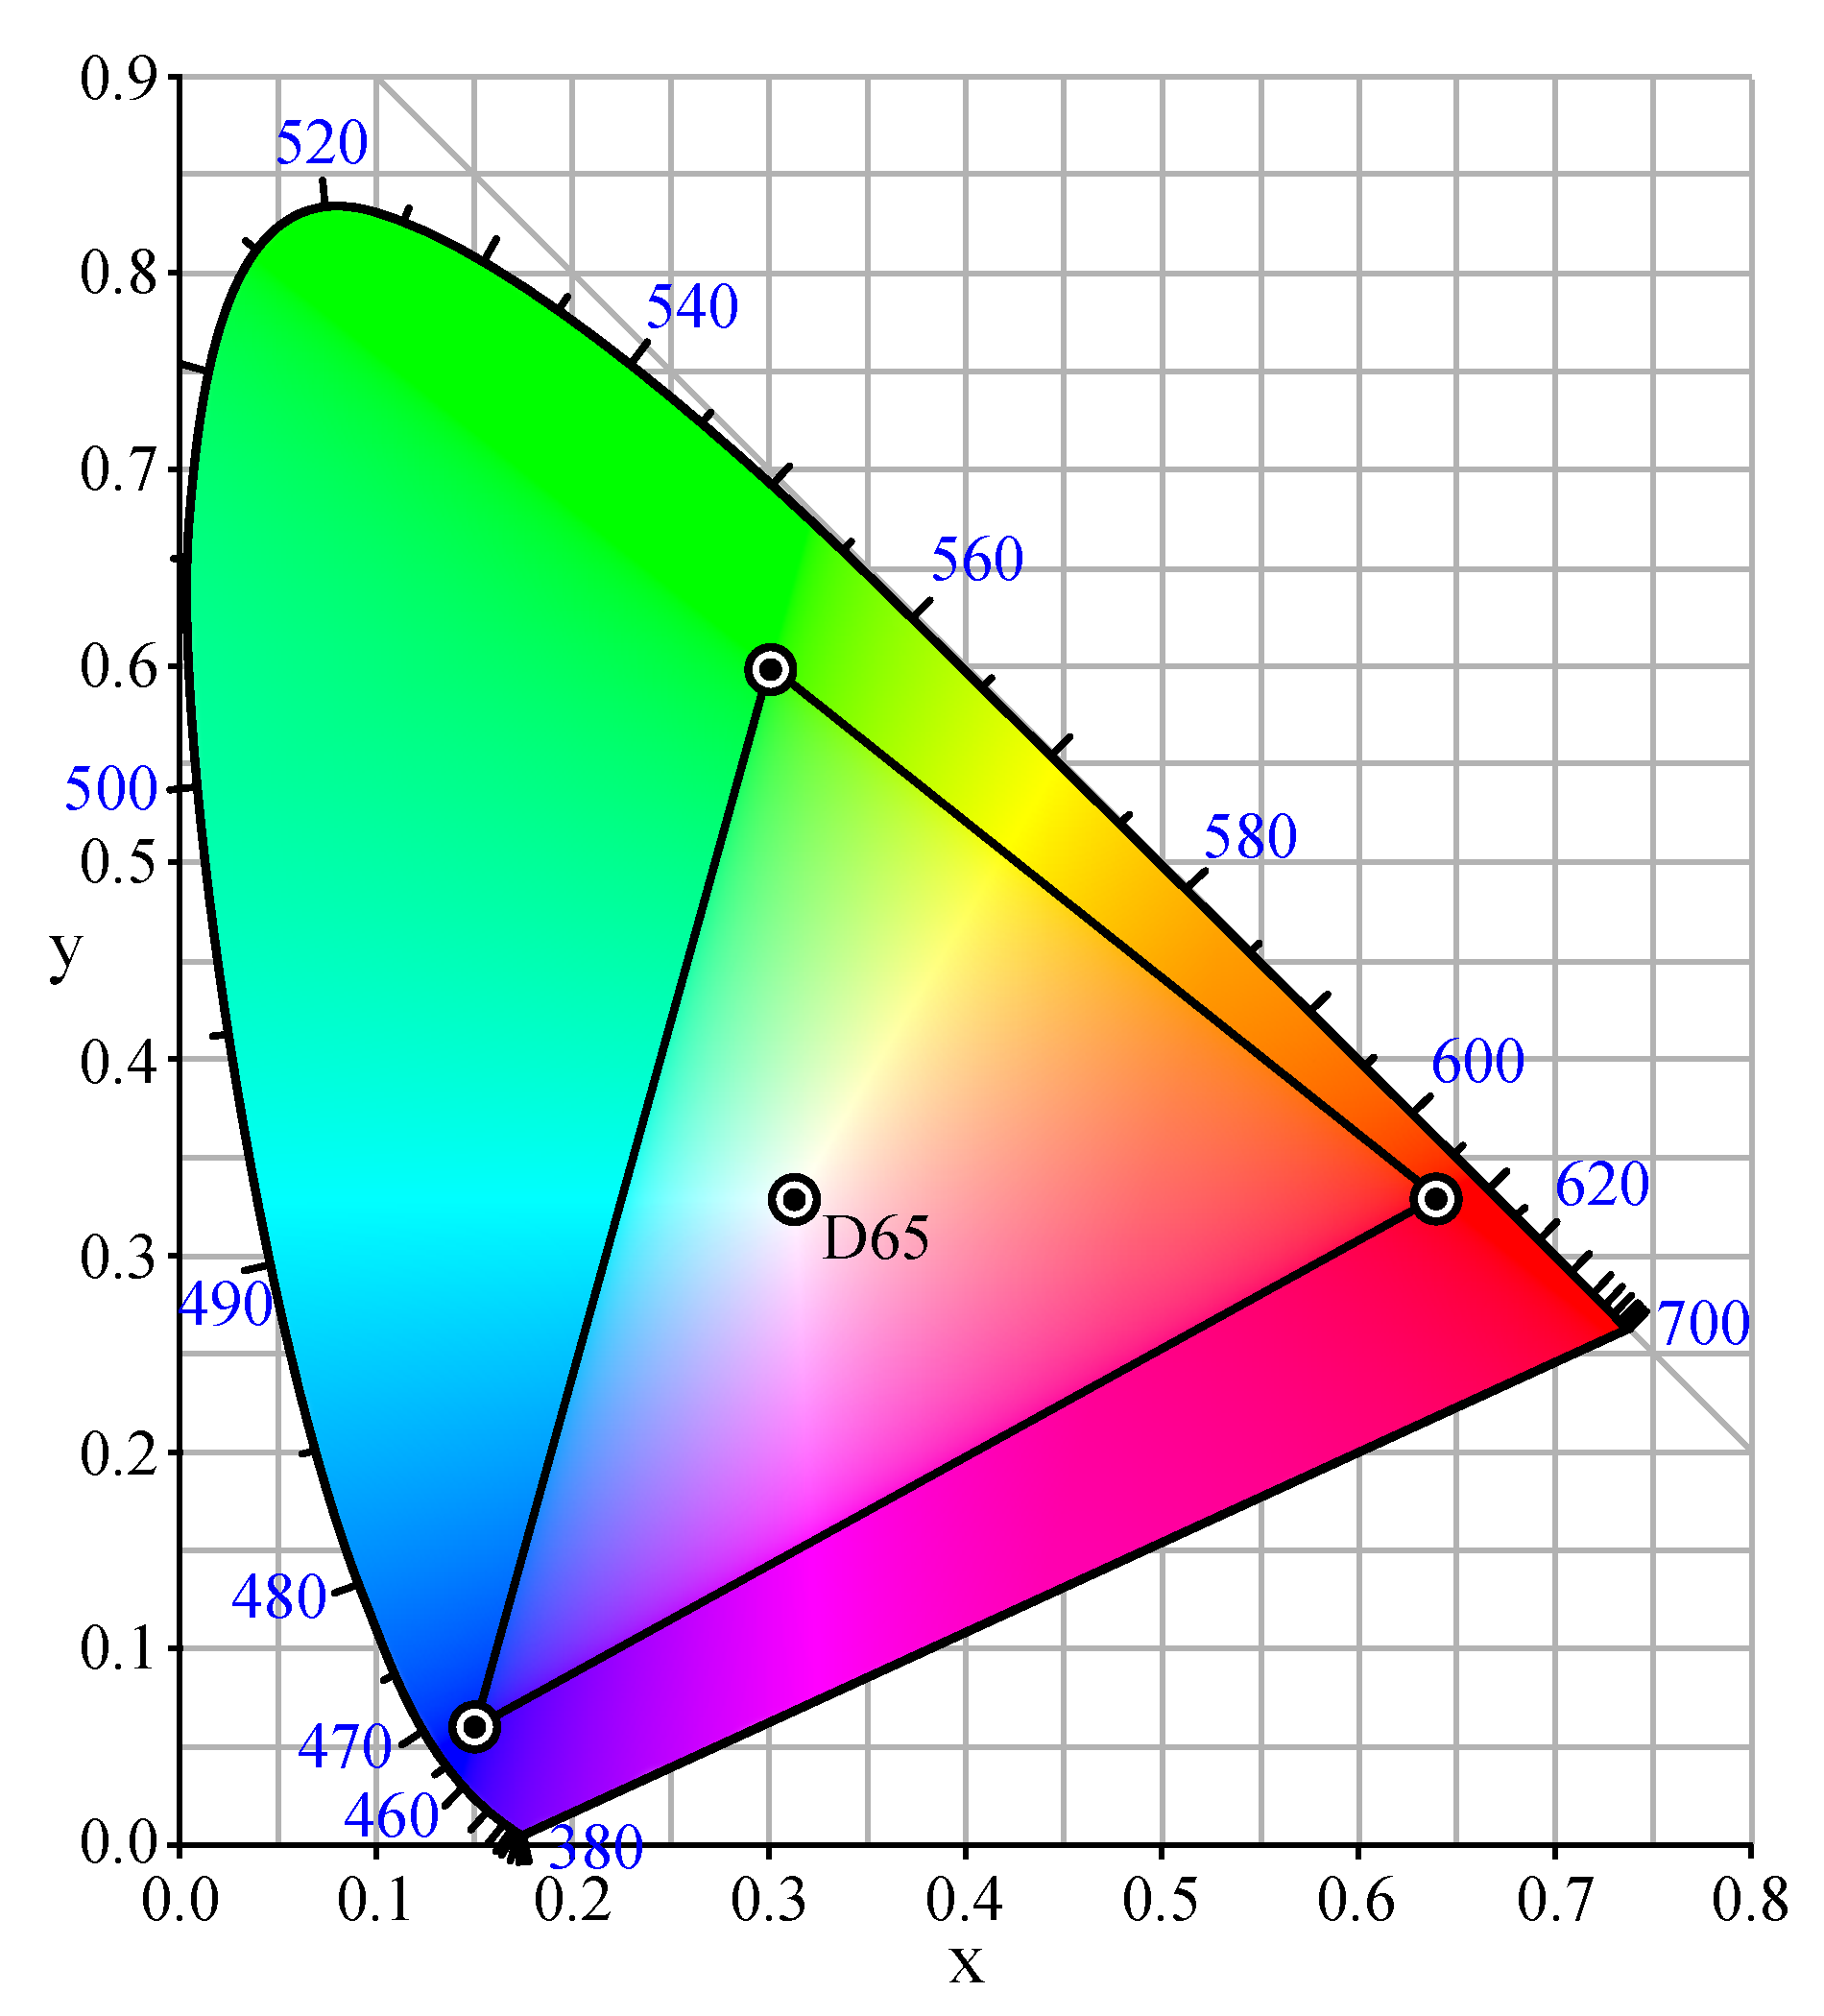
\includegraphics[width=0.95\linewidth]{fyz_fig133_rev1.pdf}
      \caption{Standardní diagram barevnosti (chromatický diagram \textbf{CIE 
       1931}\protect\footnotemark) 
              (\cite[s.~468]{Feynman01})}
      \label{fyz:fig133}
    \end{figure}
    \footnotetext{Je jeden z prvních matematicky definovaných standardů}
    Proto, rozhodneme-li se všechno zredukovat na stejnou světelnou intenzitu, můžeme použít 
    projekce na rovinu, je to provedeno na obr. \ref{fyz:fig133}. A z toho vyplývá, že libovolná 
    barva, kterou lze získat smísením dvou barev v libovolném poměru, se bude nacházet někde na 
    čáře spojující tyto dva body. Například pro stejný poměr barev bude výsledná barva ležet ve 
    středu mezi nimi a pro \num{1/4} jedné a \num{3/4} druhé bude ležet ve čtvrtině vzdálenosti od 
    první k druhé. Vezmeme-li za primární barvy modrou, zelenou a červenou, vidíme, že všechny 
    barvy, jež z nich můžeme vytvořit pomocí kladných koeficientů, leží uvnitř čárkovaného 
    trojúhelníka, jež obsahuje skoro všechny běžné barvy. Všechny možné viditelné barvy jsou totiž 
    ohraničeny zakřivenou čárou ohraničující divně tvarovanou plochu. Odkud pochází tato plocha? 
    Kdosi jednou velmi pozorně sladil všechny viditelné barvy pomocí tří speciálních barev. 
    Nemusíme ale kontrolovat všechny viditelné barvy, stačí, když si zkontrolujeme čisté spektrální 
    barvy, spektrální čáry. Libovolné světlo můžeme považovat za součet různých kladných příspěvků 
    různých čistých spektrálních barev - čistých z fyzikálního hlediska. Dané světlo bude obsahovat 
    určité množství spektrálních barev - červené, žluté, modré atd. Proto, když víme, kolik je 
    třeba každé naší primární barvy k vytvoření těchto čistých složek, můžeme vypočítat, kolik je 
    jí třeba k vytvoření dané barvy. Najdeme-li tedy barevné koeficienty všech spektrálních barev 
    pro libovolné dané tři primární barvy, můžeme sestavit celou tabulku míšení barev.

    \begin{figure}[ht!]  %\ref{fyz:fig134}
      \centering
      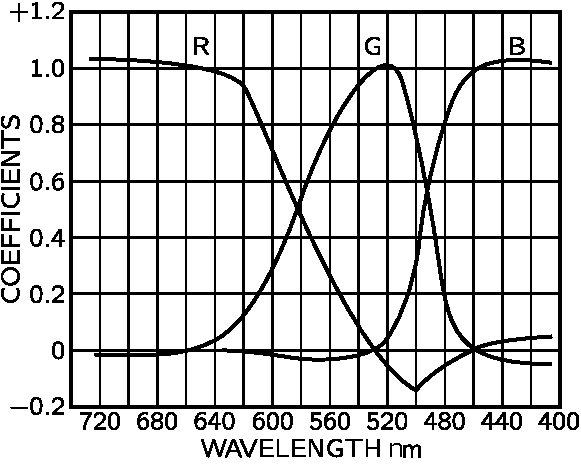
\includegraphics[width=0.9\linewidth]{fyz_fig134.pdf}
      \caption{Barevné koeficienty pro čisté spektrální barvy vyjádřené pomocí určité sady
               primárních barev. (R - červená, G - zelená, B - modrá)
              (\cite[s.~475]{Feynman01})}
      \label{fyz:fig134}
    \end{figure}
    Příklad takového experimentálního míšení barev je na obr. \ref{fyz:fig134}. Je na něm vidět, 
    jaké množství každé ze tří různých primárních barev, červené, zelené a modré, je třeba k 
    vytvoření všech spektrálních barev. Na levém konci spektra je červená, vedle je žlutá a tak až 
    po modrou. Všimněme si, že v některých bodech jsou nutná záporná znamení. Na základě takových 
    údajů je pak možné najít polohy všech barev na náčrtku, na němž jsou osy \(x\) a \(y\) dány do 
    souvislosti s množstvím různých použitých primárních barev. Takovým způsobem byly nalezeny 
    zakřivené hraniční čáry. Jsou to polohy čistých spektrálních čar. Každou libovolnou barvu lze 
    vytvořit pomocí sčítání spektrálních čar, proto vše, co lze vytvořit spojením jedné části 
    hraniční čáry s její druhou částí, odpovídá barvám přítomným v přírodě. Přímá čára spojuje 
    krajní fialový bod s krajním červeným bodem spektra. Je to poloha purpurové. Uvnitř hraničních 
    čar jsou barvy, jež lze vytvořit pomocí světel a vně barvy, jež nelze pomocí světel vytvořit, a 
    které nikdo nikdy neviděl (snad jen v halucinacích).
    
  \section{Mechanizmus barevného vidění}\label{fyz:IchapXXXVsecV}

    Další stránka problému souvisí s otázkou, proč se barvy tak chovají. Podle nejjednodušší 
    teorie, kterou navrhl Young a Helmholtz, se předpokládá, že v oku jsou tři různé pigmenty 
    citlivé na světlo, jež mají různá absorpční spektra, takže jeden pigment silně absorbuje, dejme 
    tomu, červené světlo, druhý modré a třetí zelené světlo. Když je osvítíme, nastane v těchto 
    třech oblastech různá absorpce a tyto tři části informace se v mozku nebo v oku, případně někde 
    jinde zpracovávají na výsledný barevný vjem. Snadno lze ukázat, že z těchto předpokladů by 
    vyplývala všechna pravidla míšení barev. O celé věci se mnoho debatovalo, další problém je 
    samozřejmě určit absorpční charakteristiky každého z těchto tří pigmentů. Bohužel se ukazuje, 
    že vzhledem k tomu, že barevné souřadnice lze libovolně transformovat, můžeme při experimentech 
    s míšením barev najít jen všechny možné lineární kombinace absorpčních křivek, ale ne křivky 
    pro jednotlivé pigmenty. 
    
    \begin{figure}[ht!]   %\ref{fyz:fig135}
      \centering
      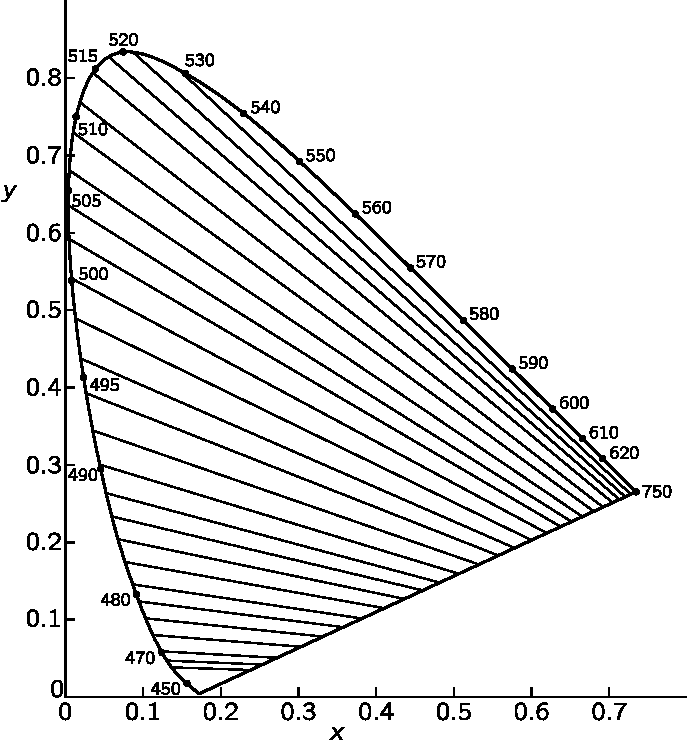
\includegraphics[width=0.9\linewidth]{fyz_fig135.pdf}
      \caption{Polohy barev zaměňovaných deuteranopy
              (\cite[s.~476]{Feynman01})}
      \label{fyz:fig135}
    \end{figure}
    Lidé se snažili různými způsoby získat určitou křivku, jež by popsala 
    nějakou fyzikální vlastnost oka. Jedna z nich se nazývá křivka jasu a je na obr. 
    \ref{fyz:fig132}. Jsou tam dvě křivky, jedna pro vidění za šera, druhá pro vidění za světla – 
    ta je křivkou jasu pro čípky. Měří se tak, že se zjišťuje, jaké je nejslabší barevné světlo, 
    jež jsme ještě schopni zaregistrovat. Určuje míru citlivosti oka v různých spektrálních 
    oblastech. Tu lze změřit i jiným zajímavým způsobem. Vezmeme-li dvě barvy, jimiž budeme 
    střídavě osvětlovat nějakou plochu a bude-li frekvence střídání barev dost nízká, budeme 
    pozorovat blikání. Budeme-li barvy střídat rychleji, při určité frekvenci, jež závisí na jasu 
    světla, blikání ustane. Může to být třeba při \num{16} opakováních za sekundu. Nyní nastavíme 
    jas nebo intenzitu obou barev tak, aby při \num{16} cyklech blikání ustalo. Abychom s takto 
    nastavenou intenzitou světla opět pozorovali blikání barev, musíme frekvenci hodně snížit. 
    Takže při vyšších frekvencích vzniká blikání jasu a při nižších frekvencích blikání barev. 
    Pomocí techniky blikání lze nastavit dvě barvy na „stejný jas“. Výsledek je téměř stejný jako 
    výsledky měření prahové citlivosti oka na vidění světla pomocí čípků. Většina pracovníků 
    používá k definici křivky jasu tuto metodu.

    \begin{figure}[ht!]  %\ref{fyz:fig136}
      \centering
      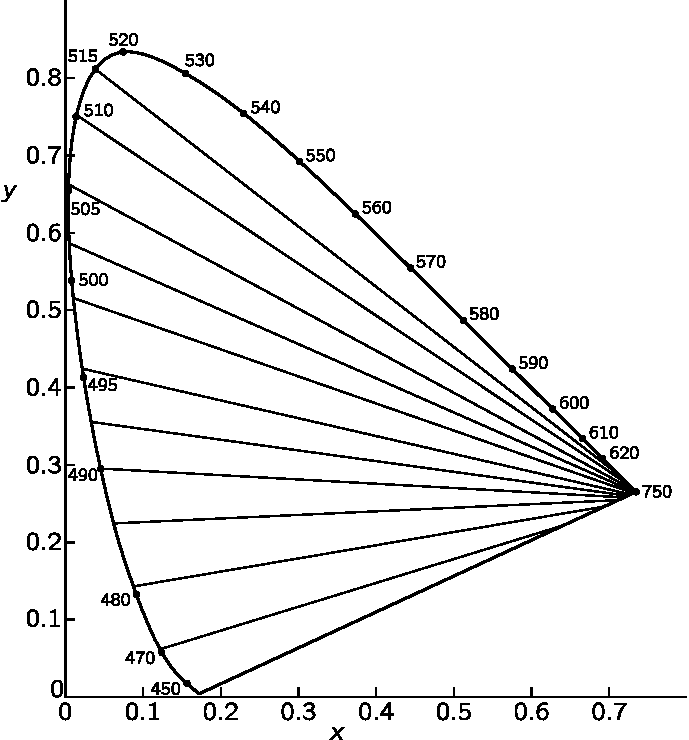
\includegraphics[width=0.9\linewidth]{fyz_fig136.pdf}
      \caption{Polohy barev zaměňovaných protanopy
              (\cite[s.~477]{Feynman01})}
      \label{fyz:fig136}
    \end{figure}
    Nacházejí-li se v oku tři pigmenty citlivé na barvy, je třeba pro každý z nich určit tvar 
    absorpčního spektra. Jak? Víme, že jsou lidé, kteří jsou barvoslepí - osm procent mužů a půl 
    procenta žen. Většina barvoslepých lidí nebo lidí s abnormálním barevným viděním mají jinou 
    míru citlivostí k různým barvám, ale k vytvoření dané barvy stále potřebují tři různé barvy. 
    Jsou však i tací, jež se nazývají dichromati a kteří získávají libovolný barevný vjem jen 
    pomocí dvou primárních barev. Vnucuje se tady myšlenka, že jim chybí jeden ze tří pigmentů. 
    Kdybychom našli tři druhy barvoslepých dichromatů, kteří mají různá pravidla míšení barev, 
    jedněm by měla chybět červená, druhým zelená a třetím modrá pigmentace. Měřením těchto tří typů 
    bychom mohli určit tři hledané křivky! Tři druhy barvoslepých dichromatů skutečně existují. Dva 
    z nich jsou dost běžné a třetí je dost vzácný. Pomocí nich se podařila určit absorpční spektra 
    pigmentů.

    \begin{figure}[ht!]  %\ref{fyz:fig137}
      \centering
      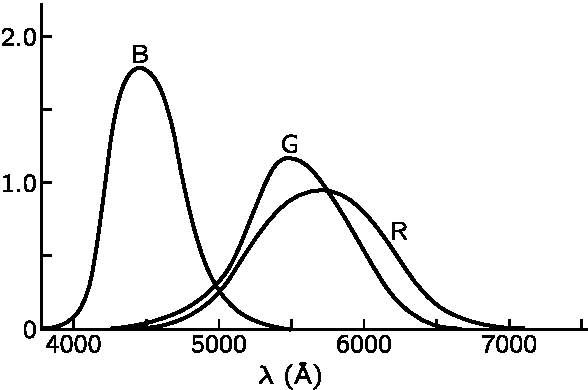
\includegraphics[width=0.9\linewidth]{fyz_fig137.pdf}
      \caption{Spektrální citlivost receptorů normálního trichromata
              (\cite[s.~477]{Feynman01})}
      \label{fyz:fig137}
    \end{figure}
    Na obr. \ref{fyz:fig135} je znázorněno míšení barev pro určitý druh barvoslepých osob, tzv. 
    deuteranopů. Pro ně nejsou polohy konstantních barev body, ale určité přímky, podél nichž se 
    jim barva jeví jako stejná. Pokud je teorie, že jim chybí jedna ze tří informací, správná, 
    všechny takové přímky by se měly protínat v jednom bodě. Když tento graf pozorně změříme, 
    zjistíme, že se dokonale protínají. Ovšem, je to proto, že graf byl sestrojen matematikem a 
    nepředstavuje skutečné údaje! Je pravda, podíváme-li se na nejnovější článek se skutečnými 
    údaji, na grafu, jako na obr. \ref{fyz:fig135}, není průsečík všech přímek na správném místě. 
    Pomocí přímek na uvedeném obrázku nemůžeme určit rozumné spektrum; potřebovali bychom negativní 
    i pozitivní absorpci pro různé oblasti. Pomocí nových údajů výzkumů Justové vychází každá z 
    absorpčních křivek všude kladná. 

    Na obr. \ref{fyz:fig136} je znázorněn jiný typ barvosleposti, tzv. protanopický typ, jenž má 
    ohnisko v blízkosti červeného konce hraniční křivky. To přibližné odpovídá i údajům Justové. 
    Pomocí tří typů barvosleposti byly nakonec definitivně určeny tři křivky citlivosti pigmentů, 
    jak jsou znázorněny na obr. \ref{fyz:fig137}.
    
  \section{Fyziochemie barevného vidění}\label{fyz:IchapXXXVsecVI}
    A což tak zkontrolovat, zda tyto křivky platí pro skutečné pigmenty v oku? Pigmenty, jež lze 
    získat ze sítnice, se většinou skládají z pigmentu nazvaného \textbf{rhodopsin} (oční purpur). 
    Jeho nejzajímavější vlastností je za prvé, že se nachází téměř u všech obratlovců a za druhé, 
    že jeho křivka citlivosti se krásně shoduje s citlivostí oka, jak vidíme na obr. 
    \ref{fyz:fig138}. Jsou tam naneseny ve stejném měřítku citlivosti rhodopsinu a oka adaptovaného 
    na tmu. Je jasné, že to je pigment, pomocí kterého vidíme za šera; oční purpur je pigment 
    tyčinek a nemá nic společného s barevným viděním. Tento fakt byl zjištěn v roce \num{1877}. V 
    roce 1958 bylo možné tvrdit, že barevné pigmenty nikdy nikdo neviděl. Od té doby \emph{Rushton} 
    pomocí jednoduchého a krásného experimentu dva z nich detekoval.

    \begin{figure}[ht!]  %\ref{fyz:fig138}
      \centering
      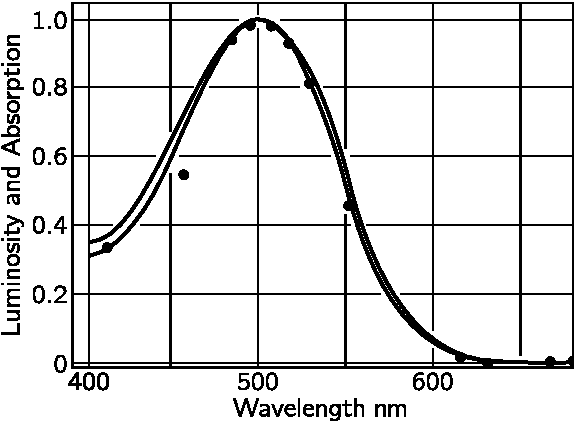
\includegraphics[width=0.8\linewidth]{fyz_fig138.pdf}
      \caption{Citlivost oka přizpůsobeného tmě v porovnání s absorpční křivkou rhodopsinu
              (\cite[s.~478]{Feynman01})}
      \label{fyz:fig138}
    \end{figure} 

    Těžkosti zřejmě spočívají v tom, že když je oko tak málo citlivé na jasné světlo ve srovnání s 
    citlivostí na nízké intenzity, potřebuje k vidění mnoho rhodopsinu, ale nepotřebuje tolik 
    barevných pigmentů k vidění barev. Rushtonova myšlenka byla ponechat pigmenty v oku a nějak je 
    změřit Provedl to následovně. Existuje přístroj nazvaný oftalmoskop, jímž se pomocí čoček vyšle 
    světlo do oka a odražené světlo přicházející zpět se soustředí do ohniska. Pomocí tohoto 
    přístroje lze zjistit, kolik světla se odrazilo zpět. Tak lze měřit koeficient odrazu světla, 
    které prošlo pigmentem dvakrát (světlo se na očním pozadí odráží a znovu prochází pigmentem 
    při návratu zpět). Příroda není vždy tak krásné organizovaná. Čípky jsou zkonstruovány tak 
    zajímavě, že světlo, které vstupuje do čípku, se odráží od stěn a postupuje dolů k malým 
    citlivým bodům ve vrcholu. Světlo jde až k citlivému bodu, odráží se a vrací zpět a opět vylétá 
    ven, takže na své cestě prochází kolem velkého množství tohoto pigmentu. Při pohledu na žlutou 
    skvrnu, kde nejsou tyčinky, nám rhodopsin situaci nekomplikuje. Ale barva sítnice byla 
    pozorována již dávno, je oranžovo - růžová, jsou v ní také krevní cévy a materiál zadní stěny 
    oka, jenž má také svou barvu. Jak víme, že se díváme na pigment? Odpověď je tato: Za prvé, 
    vezmeme si barvoslepou osobu, která má méně pigmentu a pro kterou je proto možné snadněji 
    provést analýzu. Za druhé, různé pigmenty, jako rhodopsin, mění svou intenzitu, když je 
    vyběluje světlo; při osvětlení mění svou koncentraci. Proto při sledování absorpčního spektra 
    oka osvětlil Rushton celé oko dalším světlem, které měnilo koncentraci pigmentu a měřil změnu, 
    která nastala ve spektru. Samozřejmě, že tento rozdíl nemá nic společného s množstvím krve nebo 
    s barvou odrazových vrstev apod., ale závisí jen na pigmentu. Tak Rushton získal křivku pro 
    protanopické oko, která je na obr. \ref{fyz:fig139}.

    \begin{figure}[ht!]  %\ref{fyz:fig139}
      \centering
      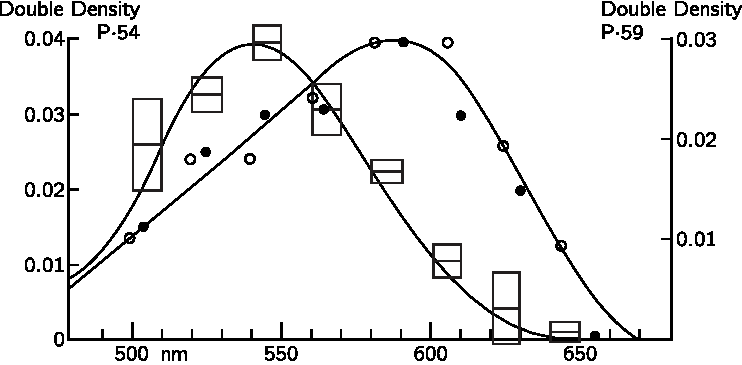
\includegraphics[width=0.8\linewidth]{fyz_fig139.pdf}
      \caption{Absorpční spektrum barevného pigmentu barvoslepého protanopa (čtverce) a normálního 
               oka (tečky)
              (\cite[s.~479]{Feynman01})}
      \label{fyz:fig139}
    \end{figure} 
    
    Druhá křivka na obr. \ref{fyz:fig139} je křivka získaná pro normální oko. Tato křivka vznikla 
    měřením normálního oka. Známe-li vlastnost jednoho pigmentu, můžeme vybělit druhý pigment 
    červeným světlem, na nějž není první pigment citlivý. Červené světlo nemá na protanopické oko 
    vliv, ale ovlivňuje normální oko, takže tak můžeme získat křivku pro chybějící pigment. Tvar 
    jedné křivky se shoduje se zelenou křivkou Justové, ale červená křivka je o něco posunuta. Snad 
    se dostáváme na správnou stopu, aleje možné, že ne, neboť poslední výzkumy s deuteranopy 
    neukazují na to, že by nějaký pigment chyběl.
    
    Otázka barvy není jen otázkou fyziky světla. Barva je vjem a \textbf{vjem} barvy se v různých 
    situacích mění. Například máme-li růžové světlo vytvořené překrýváním bílého a červeného světla 
    (růžová je jediná barva, kterou můžeme vytvořit pomocí bílé a červené), můžeme ukázat, že bílá 
    se bude zdát modrá. Postavíme-li do cesty paprskům nějaký předmět, dostaneme od něho dva stíny 
    - jeden osvětlený pouze bílým světlem a druhý pouze červeným světlem. Většině lidí se zdá, že 
    „bílý“ stín je modrý, ale když ho zvětšujeme, až pokryje celé plátno, najednou vidíme, že je 
    bílý a ne modrý! Další podobné efekty můžeme získat smísením červeného, žlutého a bílého 
    světla. Červená, žlutá a bílá mohou vytvořit pouze oranžovožluté barvy, tedy když je smísíme v 
    přibližně stejném poměru, dostaneme jen oranžové světlo. Navzdory tomu, když z těchto světel 
    vytvoříme stíny s různě překrývajícími se barvami, dostaneme celou sérii nádherných barev, 
    které tam vlastně nejsou (světlo je jen oranžové), ale jsou v našich vjemech. Jasně vidíme 
    mnoho různých barev, které jsou zcela jiné než „fyzikální“ barvy v paprsku. Velmi důležité je, 
    abychom si uvědomili, že již sítnice o světle „přemýšlí“; porovnává to, co vidí v jedné oblasti 
    s tím, co vidí v druhé, i když si to neuvědomuje. O našich poznatcích, jak to sítnice dělá, se 
    zabývá kapitola \ref{fyz:IchapXXXVI}. 
    

} %tikzset
%---------------------------------------------------------------------------------------------------
\printbibliography[heading=subbibliography]
\addcontentsline{toc}{section}{Seznam literatury}